% Task 5: ElGamal on a curve. Values from Task5/ec_elgamal.py: G = (5, 1), d = 7, Q = 7G = (0, 6), M = (13, 10), k = 4.
% CHECKED (python3, Task5/ec_elgamal.py prints Q = (0, 6)); C1, C2 and the decrypted point are the results: not shown
\documentclass[12pt,tikz,border=6pt]{standalone}
% Shared preamble of the task figures of Lecture 5 (based on Lecture2/task-figures/common.tex).
% The roles take the colours of the elliptic-curves simulator (CryptographySimulators/elliptic-curves),
% so that the README figures and the simulator look the same:
%   secret (number or point): amber, public point: violet, Alice: blue, Bob: green,
%   Eve: red, ciphertext: brown, message: grey, a change or the unknown: orange.
\usepackage{lmodern}
\usepackage[T1]{fontenc}
\renewcommand{\familydefault}{\sfdefault}
\usepackage{amsmath,amssymb}
\usepackage{xcolor}
\usepackage{fontawesome5}
\usetikzlibrary{arrows.meta, calc, positioning, fit, decorations.pathreplacing, backgrounds}

% ---------- template and neutral ----------
\definecolor{DeepBlue}{HTML}{283593}
\definecolor{AccentOrange}{HTML}{EB5A14}
\definecolor{nInk}{HTML}{37474F}
\definecolor{nLine}{HTML}{90A4AE}
\definecolor{nLight}{HTML}{CFD8DC}
\definecolor{nFill}{HTML}{ECEFF1}
\definecolor{aExec}{HTML}{43A047}
\definecolor{aWrite}{HTML}{E53935}

% ---------- roles (the colours of the elliptic-curves simulator) ----------
\definecolor{rPriv}{HTML}{E2A60E}  \definecolor{rPrivBg}{HTML}{FDF3DC}  \definecolor{rPrivText}{HTML}{9A6B00}
\definecolor{rPub}{HTML}{8A5CD8}   \definecolor{rPubBg}{HTML}{F1EAFD}   \definecolor{rPubText}{HTML}{6A3FB8}
\definecolor{rAli}{HTML}{2F6FDB}   \definecolor{rAliBg}{HTML}{E5EDFB}
\definecolor{rBob}{HTML}{2FA84F}   \definecolor{rBobBg}{HTML}{E3F4E8}   \definecolor{rBobText}{HTML}{1E7E4F}
\definecolor{rEve}{HTML}{E5484D}   \definecolor{rEveBg}{HTML}{FDE9E9}
\definecolor{rCip}{HTML}{A8642A}   \definecolor{rCipBg}{HTML}{F7ECE0}
\definecolor{rMsg}{HTML}{BCC4CC}   \definecolor{rMsgBg}{HTML}{EEF1F4}
\definecolor{rChg}{HTML}{D9621C}   \definecolor{rChgBg}{HTML}{FCE8DA}

\tikzset{
  hw/.style={draw=nLine, thick, fill=nFill, text=nInk, rounded corners=3pt, align=center, inner sep=4pt},
  hwmain/.style={draw=nInk, thick, fill=nInk, text=white, rounded corners=3pt, align=center, inner sep=4pt},
  role/.style={draw=#1, thick, fill=#1Bg, text=nInk, rounded corners=3pt, align=center, inner sep=5pt},
  unk/.style={draw=rChg, thick, dashed, fill=white, text=rChg, rounded corners=3pt, align=center, inner sep=5pt,
    font=\bfseries},
  data/.style={-{Stealth}, very thick, nInk},
  note/.style={font=\small, text=nInk},
  person/.style={circle, fill=#1, draw=#1, text=white, minimum size=1.1cm, font=\Large, inner sep=0pt},
}
\newcommand{\personnode}[4]{%
  \node[person=#3] (#1) at (#2) {\faUser};
  \node[font=\small\bfseries, text=#3, below=0.06cm of #1] (#1lbl) {#4};}
\newcommand{\cogbox}[4]{%
  \node[hwmain, minimum width=#4, minimum height=1.1cm] (#1) at (#2) {};
  \node[text=white, font=\large, anchor=west] at ([xshift=0.2cm]#1.west) {\faCogs};
  \node[text=white, font=\small\bfseries] at ([xshift=0.3cm]#1.center) {#3};}

% ---------- the toy curve y^2 = x^3 + 2x + 2 mod 17 (as on the slides) ----------
% CHECKED: python3, all (x, y) with 0 <= x, y < 17 and y^2 = x^3 + 2x + 2 mod 17: these 18 points
\newcommand{\curvepts}{0/6,0/11,3/1,3/16,5/1,5/16,6/3,6/14,7/6,7/11,9/1,9/16,10/6,10/11,13/7,13/10,16/4,16/13}
% the grid of dots, in grid coordinates (1 unit = one step of x or y); draw it inside a scope
\newcommand{\gridbody}{%
  \foreach \x in {0,...,16} \foreach \y in {0,...,16} \fill[nLight] (\x,\y) circle (1.1pt);
  \draw[nLine, thick] (-0.7,-0.7) -- (16.7,-0.7);
  \draw[nLine, thick] (-0.7,-0.7) -- (-0.7,16.7);
  \foreach \v in {0,...,16} {
    \node[font=\tiny, text=gray, anchor=north] at (\v,-0.75) {\v};
    \node[font=\tiny, text=gray, anchor=east] at (-0.75,\v) {\v};
  }
  \node[font=\scriptsize, text=nInk, anchor=west] at (16.8,-0.7) {$x$};
  \node[font=\scriptsize, text=nInk, anchor=south] at (-0.7,16.8) {$y$};
  \foreach \x/\y in \curvepts \fill[nInk] (\x,\y) circle (3pt);}
% mark a point of the grid: \gmark[colour]{x,y}{label}{where the label goes}
\newcommand{\gmark}[4][rPub]{%
  \node[circle, draw=#1, line width=1.2pt, fill=#1, minimum size=9pt, inner sep=0pt] at (#2) {};
  \node[font=\scriptsize\bfseries, text=#1, #4, inner sep=1pt, outer sep=3pt, fill=white, fill opacity=0.85,
    text opacity=1, rounded corners=1pt] at (#2) {#3};}

\begin{document}
\pagecolor{white}
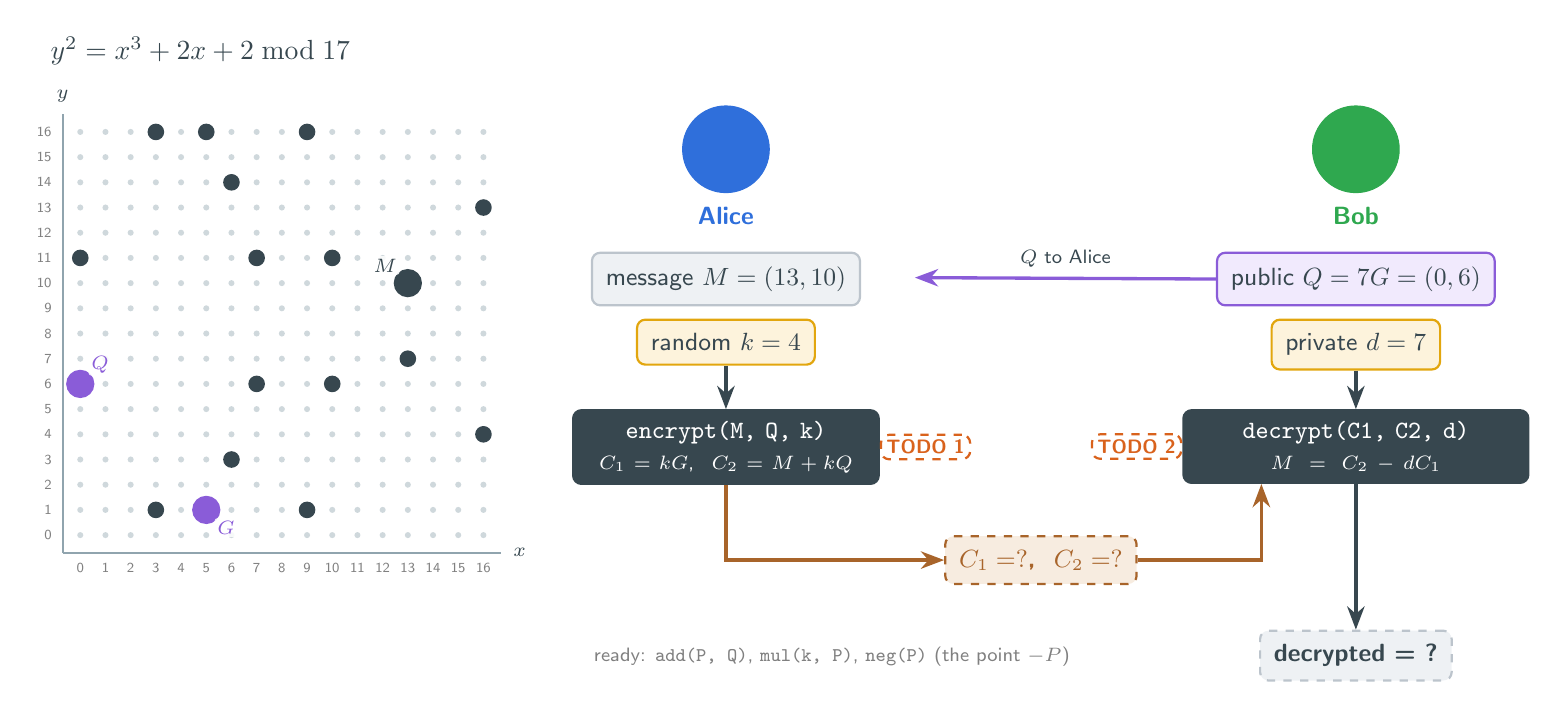
\begin{tikzpicture}[>=Stealth]
  % the curve with the known points
  \node[font=\normalsize\bfseries, text=nInk, anchor=west] at (-0.5,6.15) {$y^2 = x^3 + 2x + 2 \bmod 17$};
  \begin{scope}[x=0.32cm, y=0.32cm]
    \gridbody
    \gmark{5,1}{$G$}{below right}
    \gmark{0,6}{$Q$}{above right}
    \gmark[nInk]{13,10}{$M$}{above left}
  \end{scope}

  % the flow
  \begin{scope}[shift={(7.6,0)}]
    \personnode{alice}{0.6,4.9}{rAli}{Alice}
    \personnode{bob}{8.6,4.9}{rBob}{Bob}
    \node[role=rMsg, font=\small, anchor=north] (m) at (0.6,3.6) {message $M = (13, 10)$};
    \node[role=rPriv, font=\small, anchor=north] (k) at (0.6,2.75) {random $k = 4$};
    \node[role=rPriv, font=\small, anchor=north] (d) at (8.6,2.75) {private $d = 7$};
    \node[role=rPub, font=\small, anchor=north] (q) at (8.6,3.6) {public $Q = 7G = (0, 6)$};
    \draw[data, rPub] (q.west) -- node[above, font=\scriptsize, text=nInk] {$Q$ to Alice} (3.0,3.27);
    % encrypt
    \node[hwmain, font=\small\ttfamily, text width=3.6cm, anchor=north] (enc) at (0.6,1.6)
      {encrypt(M, Q, k)\\ \normalfont\scriptsize $C_1 = kG$, \ $C_2 = M + kQ$};
    \node[unk, font=\scriptsize\bfseries, anchor=west, inner sep=2pt] at (enc.east) {TODO 1};
    \draw[data] (k.south) -- (enc.north);
    % ciphertext
    \node[unk, draw=rCip, text=rCip, fill=rCipBg, font=\small\bfseries, anchor=north] (c) at (4.6,0.0) {$C_1 = ?$, \ $C_2 = ?$};
    \draw[data, rCip] (enc.south) |- (c.west);
    % decrypt
    \node[hwmain, font=\small\ttfamily, text width=4.1cm, anchor=north] (dec) at (8.6,1.6)
      {decrypt(C1, C2, d)\\ \normalfont\scriptsize $M = C_2 - dC_1$};
    \node[unk, font=\scriptsize\bfseries, anchor=east, inner sep=2pt] at (dec.west) {TODO 2};
    \draw[data] (d.south) -- (dec.north);
    \draw[data, rCip] (c.east) -| ([xshift=-1.2cm]dec.south);
    \node[unk, font=\small\bfseries, draw=rMsg, text=nInk, fill=rMsgBg, anchor=north] (out) at (8.6,-1.2) {decrypted = ?};
    \draw[data] (dec.south) -- (out.north);
    \node[font=\scriptsize, text=gray, anchor=north west, align=left] at (-1.2,-1.3)
      {ready: \texttt{add(P, Q)}, \texttt{mul(k, P)}, \texttt{neg(P)} (the point $-P$)};
  \end{scope}
\end{tikzpicture}
\end{document}
